\chapter{Системы управления синхронными двигателями с постоянными магнитами} \label{ch:ch2}

\section{Методы математического описания} \label{sec:ch2/sec1}
Для синхронных машин с постоянными магнитами характерны значительный воздушный зазор и низкая степень насыщения. Поэтому при их рассмотрении часто используются модели без учета нелинейности магнитной цепи.
В модель синхронного электромеханического преобразователя без учета насыщения вводится ряд допущений, позволяющих применить принцип суперпозиции к описанию магнитных полей от различных источников и обеспечить понимание основных закономерностей преобразования энергии в
этой машине:
\begin{enumerate}
\item Магнитно-мягкий материал магнитопровода имеет
бесконечную магнитную проницаемость;
\item Отсутствие насыщения делает все сосредоточенные электрические параметры независимыми от электрических
переменных;
\item Реальные обмотки и постоянные магниты заменяются эквивалентными токовыми слоями, создающими требуемое значение и форму напряженности или магнитодвижущих сил магнитного поля в равномерном воздушном зазоре машины;
\item Запасенная магнитная энергия, используемая для описания электрической машины, рассматривается лишь как энергия статического магнитного поля;
\item Энергия электростатического поля считается пренебрежимо
малой;
\item Электрические поля, возникающие при изменении во времени магнитных полей или относительном движении в магнитном поле, не учитываются при вычислении запасенной магнитной энергии; они появляются при выводе дифференциальных уравнений движения машины;
\item Краевые эффекты на границах зубцовых зон (явно выраженных полюсов) отсутствуют;
\item Постоянный магнит является идеальным источником напряженности магнитного поля и представляет собой бесконечно тонкую пластину;
\item Потери в стали отсутствуют;
\item Магнитная проницаемость воздушного зазора представляется в виде произведения магнитной проницаемости статора и ротора [12].
\end{enumerate}

Последнее допущение требует пояснений. В общем случае предполагается, что зубчатые структуры имеются на внутренней стороне цилиндрического статора и внешней поверхности цилиндрического ротора. Тогда относительная магнитная проницаемость воздушного зазора между зубчатой структурой
статора и поверхностью ротора $\mu_{1}$ аппроксимируется в предположении, что поверхность ротора гладкая:
\begin{equation}
\label{eq:mu1}
\mu_{1}=\mu_{10}+\sum_{k=1}^{\infty} \mu_{1 k} \cos k \theta_{1}
\end{equation}

Для зубчатой структуры ротора относительная магнитная проницаемость воздушного зазора между зубчатой структурой ротора и поверхностью статора $\mu_{2}$ определяется в предположении гладкой рабочей поверхности статора:
\begin{equation}
\label{eq:mu2}
\mu_{2}=\mu_{20}+\sum_{l=1}^{\infty} \mu_{1 l} \cos k \theta_{2}
\end{equation}

\section{Существующие системы управления электроприводом на базе синхронного двигателя с постоянными магнитами
} \label{sec:ch2/sec1}

\subsection{Полеориентированное управление электроприводом на базе синхронного двигателя с постоянными магнитами}
Основные принципы полеориентированного управления были разработаны в 70-х годах девятнадцатого века. Сегодня в результате фундаментальных теоретических исследований и успехов в области силовой полупроводниковой электроники и микропроцессорных систем разработаны электроприводы с векторным управлением, которые серийно выпускаются электротехническими фирмами всего мира. 
Если под скалярным регулированием скорости понимается такое регулирование, при котором в качестве переменных в системе используются эффективные значения напряжений, токов и потокосцеплений, а сами эти величины считаются величинами скалярными, то в основе полеориентированного управления лежит представление об этих величинах, как о пространственных векторах. Можно также отметить, что скалярное управление базируется на зависимостях, лежащих в основе схемы замещения двигателя, а векторное управление — на соответствующих структурных схемах. [35, 27, 117]. 
Для пояснения смысла использования векторного управления обратимся к математическому описанию синхронного двигателя в пространственных векторах при ориентации вещественной оси вращающейся системы координат $d-q$ по вектору ${\Psi }_{2}$ . Такому описанию соответствуют формулы \labelcref{eq:PMSMdqMw} вместе с равенством $\omega_{2эл}=\frac{d \theta_{2}}{d t}$ , выражением для электромагнитного момента и основным уравнением механики. 

\begin{equation}
\label{eq:PMSMdqMw}
\begin{multlined}
\begin{cases}
U_{1 d}=R_{1} i_{1 d}+p\left(L_{1 d} i_{1 d}+\Psi_{2}\right)-\omega_{r} z_{\text{п}}\left(L_{1 q} i_{1 q}\right)
\\
U_{1 q}=R_{1} i_{1 q}+p L_{1 q} i_{1 q}+\omega_{r} z_{\text{п}}\left(L_{1 d} i_{1 d}+\Psi_{2}\right)
\\
M_{\text{э}}=\frac{3}{2} z_{\text{п}}\left(\psi_{1 d} i_{1 q}-\psi_{1 q} i_{1 d}\right)
\\
\frac{d \omega_{r}}{d t}=\frac{1}{J}\left(M_{\text{э}}-M_{\text{с}}\right)
\end{cases}	
\end{multlined}
\end{equation}
где: $\psi_{2 a}=\Psi_{2} \cos \omega t$; $\psi_{2 \beta}=\Psi_{2} \sin \omega t$; $\psi_{1 \alpha}=L_{1} \cdot i_{1 \alpha}+\psi_{2 \alpha}$; $\psi_{1 \beta}=L_{1} \cdot i_{1 \beta}+\psi_{2 \beta}$; $U_{1 \alpha}, U_{1 \beta}, i_{1 \alpha}, i_{1 \beta}, \psi_{1 \alpha}, \psi_{2 \alpha}, \psi_{2 \beta}$ - составляющие векторов напряжений, токов, потокосцеплений по осям $\alpha$ и $\beta$; $r_{1}$, $L_{1}$ - сопротивление, и индуктивность статорной обмотки; $J$ - момент инерции ротора; $\omega_{r}$ – угловая частота вращения ротора; $z_{\text{п}}$ - число пар полюсов двигателя; $M_{\text{э}}$ и $M_{\text{с}}$ - электромагнитный момент и момент статической нагрузки.

\begin{figure}[ht]
	\centering
	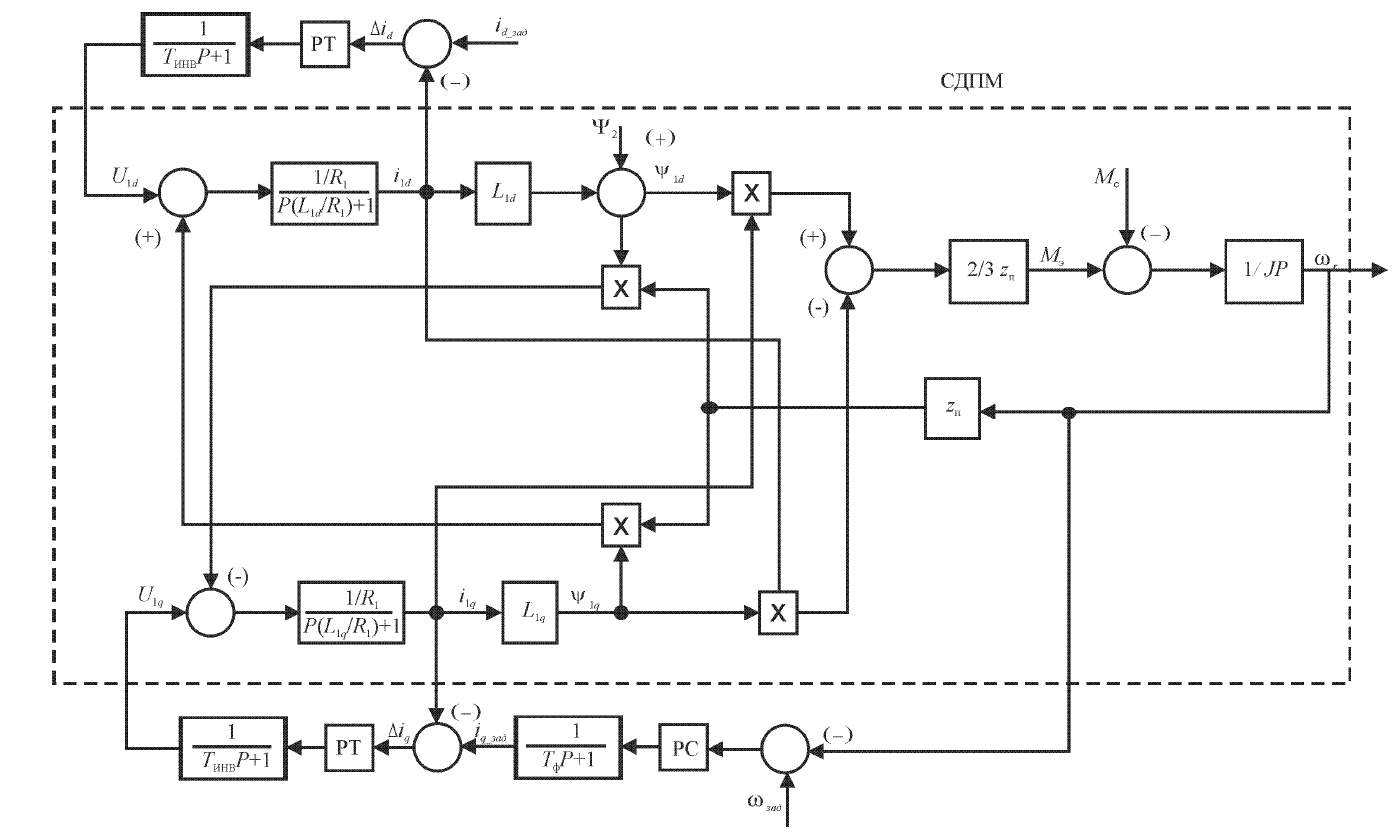
\includegraphics [scale=0.5] {FOCPMSM}
	\caption{Структурная схема электропривода при полеориентированном управлении на базе СДПМ}
	\label{fig:FOCPMSM}
\end{figure}

По этим формулам построена Структурная схема синхронного двигателя (рис. \ref{fig:FOCPMSM}), в которой все переменные представлены сигналами постоянного тока. Входными сигналами являются проекции вектора статорного напряжения $u_{1 d}$ и $u_{1q}$, а выходными величинами электромагнитной части схемы — потокосцепление ротора ${\Psi }_{2}$ и электромагнитный момент $M_{\text{э}}$ . Частота роторной ЭДС $\omega_{r}$ рассчитывается через проекцию на ось $q$ вектора тока статора и потокосцепление ротора. В свою очередь, через скорость двигателя $\omega$ и роторную частоту $\omega_{r}$ рассчитывается частота напряжения обмотки статора $\omega_{\text{эл}}$. В структуре двигателя существуют перекрестные связи между каналом формирования потокосцепления ротора и каналом формирования электромагнитного момента.

Если тем или другим способом скомпенсировать влияние перекрестных связей, то окажется, что сигналом по оси $d$ независимо задается потокосцепление ротора, а сигналом по оси $q$ электромагнитный момент при данном значении потокосцепления ротора ${\Psi }_{2}$. 
Таким образом, структура синхронного двигателя, полученная на основе рассмотрения пространственных векторов, оказывается практически такой же, как структура двигателя постоянного тока независимого возбуждения.
Аналогия с двигателем постоянного тока становится еще более очевидной, если в преобразователе, от которого питается двигатель, с помощью быстродействующих токовых контуров формируются непосредственно составляющие тока статора $i_{1 d}$ и $i_{1 q}$. Улучшение динамических свойств электропривода с синхронным двигателем при векторном управлении является результатом того, что в переходных процессах имеется возможность поддерживать постоянство потокосцепления ротора, в отличие от скалярного регулирования, где потокосцепление ротора в переходных процессах меняется при изменении токов статора и ротора, что приводит к снижению темпа изменения электромагнитного момента. В приводе с полеориентированном управлением, где потокосцепление ротора можно поддерживать постоянным, электромагнитный момент изменяется так быстро, как быстро изменяется составляющая тока статора $i_{1 q}$, (аналогия с изменением момента при изменении тока якоря $i_{\text{я}}$ в машине постоянного тока). 
При первой трактовке [31] к системам с прямой ориентацией по полю относят только те системы, в которых осуществляется непосредственное измерение потока с помощью тех или иных датчиков потока. Вторая трактовка [10, 117] относит к системам с прямой ориентацией и те системы, в которых поток рассчитывается по модели двигателя, так как это даёт возможность, так же как при непосредственном измерении потока, построить замкнутый контур его регулирования. К системам с косвенным измерением в этом случае относят только системы, в которых поток не измеряется и не рассчитывается, а формируется путём задания других переменных. 
Система с косвенной ориентацией по полю не содержит узлов измерения или расчета потокосцепления ротора. Требуемые сигналы задания составляющих тока статора формируются на основании заданных значений потокосцепления ${\Psi }_{2}$ электромагнитного момента. 
Как уже отмечалось, структурная схема синхронного двигателя во вращающейся системе координат содержит в качестве входных и выходных величин проекции соответствующих пространственных векторов на оси вращающейся системы координат. Эти величины являются величинами постоянного тока, что позволяет строить систему управления электроприводом так же, как систему управления электроприводом постоянного тока. Между тем, в реальной системе с трехфазным синхронным двигателем напряжения и токи представляют собой трехфазные системы синусоидальных величин. Поэтому при построении системы управления электроприводом на основе функциональной схемы рис. 2.7. должны быть введены преобразователи координат, осуществляющие преобразование величин постоянного тока во вращающейся системе координат в трехфазную систему величин в неподвижной системе координат и обратно.

\subsection{Прямое управление моментом электроприводом на базе синхронного двигателя с постояными магнитами}

В исследуемой системе прямого управления моментом
СДПМ лежит метод управления моментом и потоком с помощью
предельных циклов путём подачи с выхода инвертора на вход
СДПМ оптимального напряжения.

\noindent Достоинства метода:
\begin{itemize}
	\item хорошие динамические свойства;
	\item простое исполнение.
	\item нет необходимости в использовании прямого преобразователя
	координат, а используется упрощенный обратный преобразователь
	координат;
	\item нет необходимости в использовании датчика скорости;
	\item свойства синхронного электропривода подобны электроприводу постоянного тока с двигателем независимого
	возбуждения
\end{itemize}

\noindent Недостатки метода:
\begin{itemize}
	\item изменяющаяся частота переключения;
	\item точность регулирования определяется используемой моделью двигателя;
	\item большие пульсации токов и момента;
	\item при малых скоростях не обеспечивается стабильный режим
	работы;
	
\end{itemize}

Прямое управление моментом является продолжением и развитием векторного подхода к построению систем управления асинхронным двигателем. Принципы такого управления были опубликованы в 1985 г. и через 10 лет появились первые сообщения о промышленных образцах систем управления фирмы АВВ, построенных на этих принципах.
Задачей прямого управления моментом является обеспечение быстрой реакции электромагнитного момента двигателя на управляющее воздействие. В отличие от полеориентированного управления, где изменение момента производится путем воздействия на ток статора, который, таким образом, является управляемой величиной, в системе с прямым управлением моментом управляемой величиной является потокосцепление статора [1, 2]. Изменение потокосцепления достигается путем оптимального переключения ключей инвертора напряжения, от которого питается синхронный двигатель  (рис. \ref{fig:PMSMDTC}). 

\begin{figure}[ht]
	\centering
	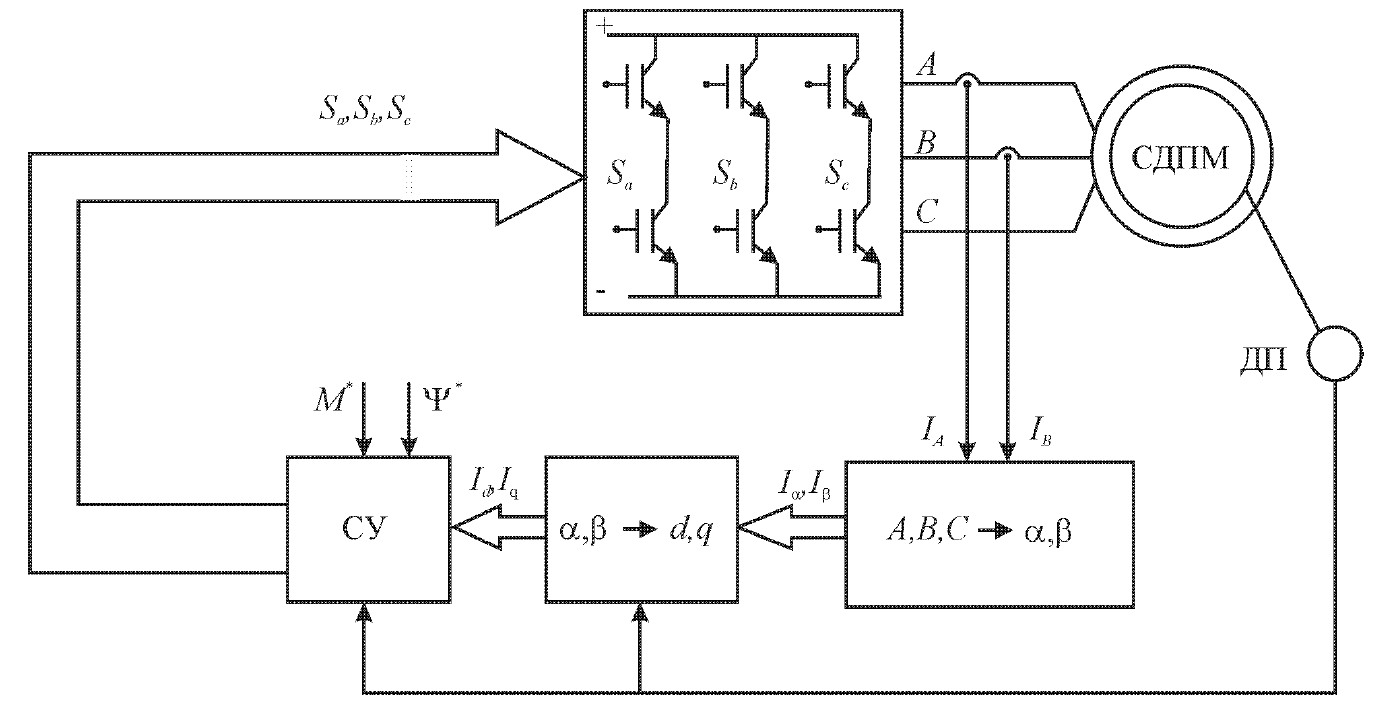
\includegraphics [scale=0.5] {PMSMDTC}
	\caption{Структурная схема электропривода при полеориентированном управлении на базе СДПМ}
	\label{fig:PMSMDTC}
\end{figure}

Для рассмотрения принципа прямого управления моментом [117] могут быть использованы два полученных ранее выражения: уравнение равновесия напряжений статорной цепи в неподвижной системе координат (формула \ref{eq:U1dq}) и выражение \ref{eq:Mel} для электромагнитного момента двигателя. 
\begin{equation}
\label{eq:U1dq}
\overline{U}_{\mathrm{ldq}}=R_{1} \overline{I}_{\mathrm{ldq}}+\frac{d}{d t} \overline{\Psi}_{\mathrm{ldq}}
\end{equation}
\begin{equation}
\label{eq:Mel}
\vec{M}_{\text{э}}=L_{1}\left(\vec{\Psi}_{1} \Psi_{2}^{*}\right)
\end{equation}
Это выражение, в котором момент рассчитывается через потокосцепления статора и ротора, записано во вращающейся системе координат d-q, но поскольку значение момента не зависит от выбора системы координат, в которой рассматриваются векторы $\overline{\Psi}_{1}$ и $\overline{\Psi}_{2}$ , то оно может быть представлено в неподвижной системе координат $d-q$ в виде:
\begin{equation}
M_{\text{э}}=\frac{3}{2} z_{\text{п}} L_{1}\left(\psi_{1 q} \psi_{2 d}-\psi_{1 d} \psi_{2 q}\right)
\end{equation}

На рис. \ref{fig:VectorPMSM} [3, 117] показана координатная плоскость, на которой отмечены оси неподвижной системы координат $d-q$ и расположение векторов напряжения и потокосцепления статора. Плоскость поделена на шесть секторов I — VI по 60 эл. град каждый.

\begin{figure}[ht]
	\centering
	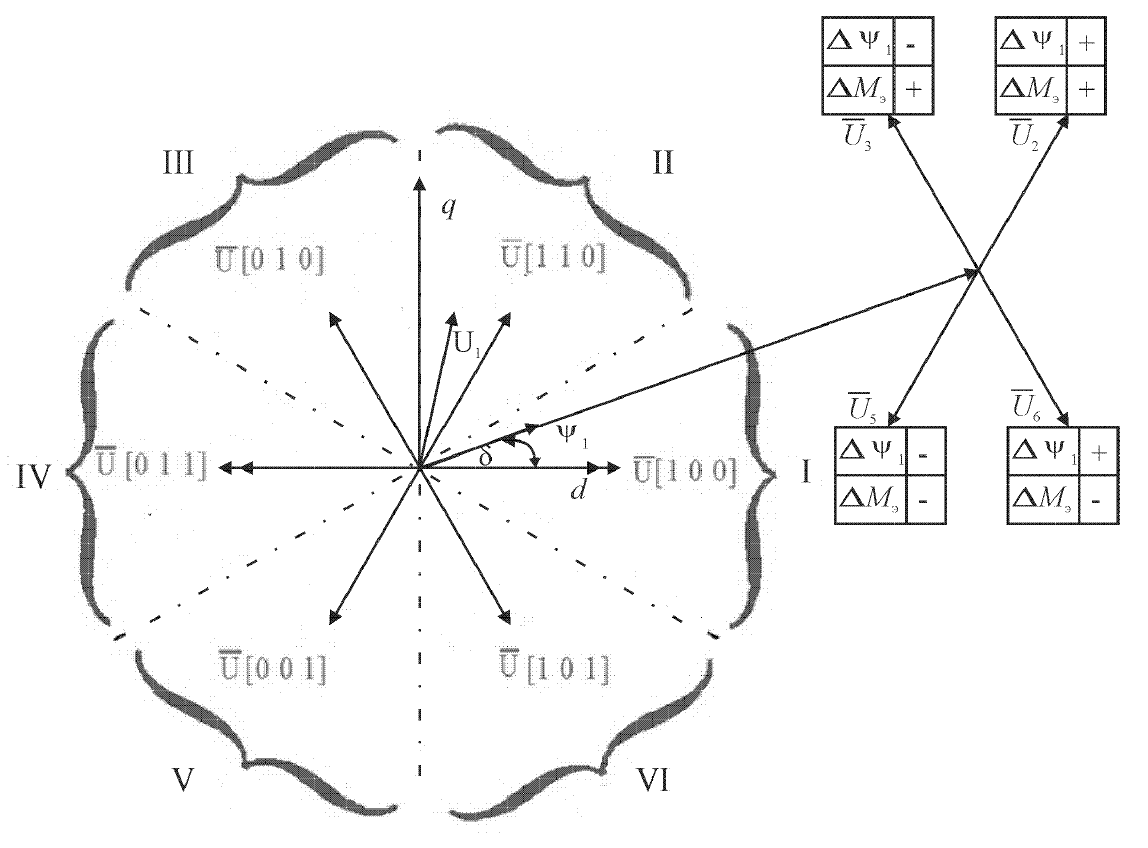
\includegraphics [scale=0.5] {VectorPMSM}
	\caption{Структурная схема электропривода при полеориентированном управлении на базе СДПМ}
	\label{fig:VectorPMSM}
\end{figure}

Пространственный вектор напряжения на выходе инвертора, от которого питается обмотка статора двигателя, может занимать одно из шести фиксированных ненулевых положений и два
нулевых положения. Ненулевые векторы $\overline{U}_{1}-\overline{U}_{6}$ и нулевые, обозначаемые, как $\overline{U}_{7}-\overline{U}_{7}$ , рассматриваются как самостоятельные базовые векторы. На рис. \ref{fig:VectorPMSM} показано мгновенное положение вектора потокосцепления статора, который в данный момент времени находится в секторе I.

Таким образом, для организации прямого управления моментом необходимо знать текущие значения потокосцепления статора и момента двигателя.

Для расчета значений потокосцепления статора и электромагнитного момента необходимо располагать проекциями векторов тока и напряжения в системе координат $d-q$. Поэтому в модели выполняется преобразование симметричной трехфазной системы токов и напряжений в проекции соответствующих векторов на оси неподвижной системы координат (см. рис. \ref{fig:VectorPMSM}). 
Сравнительный анализ электроприводов на базе синхронного двигателя с постоянными магнитами с системой полеориентированного управления и системой прямого управления
моментом показал, что обе системы управления применимы в электроприводах при различных требованиях к показателям регулируемого электропривода в различных режимах работы со стороны технологического процесса [1].
